% fig_arch.tex  -  detailed AsymVerify system-architecture figure.
% Three delineated stages (base classifier -> confidence gate -> asymmetric
% verification) with real notation, a structured-output cross-section, and the
% nine-subtype evasion taxonomy typeset as a formal clarity map.
% Wide (~3.3:1); embedded full-width on the A0 poster.
%
% NB: TikZ node alignment needs every \\ at the top level of the node body.
%     Do not nest \\ inside a {\footnotesize ...} group -- wrap each line instead.
%     (An `aligned' math block carries its own \\; that is fine inside one line.)
\documentclass[border=2mm]{standalone}
% common.tex  -  shared preamble for AsymVerify standalone figures.
% Times (ACL house face) + the poster palette + flow-diagram styles.
% Used by each fig_*.tex:  \documentclass[border=2mm]{standalone}% common.tex  -  shared preamble for AsymVerify standalone figures.
% Times (ACL house face) + the poster palette + flow-diagram styles.
% Used by each fig_*.tex:  \documentclass[border=2mm]{standalone}% common.tex  -  shared preamble for AsymVerify standalone figures.
% Times (ACL house face) + the poster palette + flow-diagram styles.
% Used by each fig_*.tex:  \documentclass[border=2mm]{standalone}\input{common.tex}
\usepackage[T1]{fontenc}
\usepackage{lato}
\usepackage{newtxmath}
\renewcommand{\familydefault}{\sfdefault}
\usepackage{amsmath}
\usepackage{tikz}
\usetikzlibrary{arrows.meta,positioning,calc,backgrounds,fit,shapes.geometric,shapes.misc}
\usepackage{xcolor}

% ---- Palette (must match beamerthemeAsymVerify.sty) ----
\definecolor{purpleDeep}{HTML}{3B2A6B}
\definecolor{purpleBrand}{HTML}{5B3C9E}
\definecolor{violetA}{HTML}{7E5BC2}
\definecolor{lavender}{HTML}{ECE7F7}
\definecolor{lavenderTwo}{HTML}{DCD2F0}
\definecolor{inkA}{HTML}{211B33}
\definecolor{passOne}{HTML}{3F4DA8}
\definecolor{passTwo}{HTML}{D24B7A}
\definecolor{passThree}{HTML}{2E9E6B}
\definecolor{goldA}{HTML}{E8B53A}
\definecolor{paperBG}{HTML}{FBFAFE}
\definecolor{slateA}{HTML}{8C86A0}
\colorlet{crColor}{passThree}
\colorlet{ambColor}{purpleBrand}
\colorlet{cnrColor}{passTwo}

% ---- Flow-diagram node + edge styles ----
\tikzset{
  io/.style   ={rounded corners=3mm, draw=violetA,   line width=1.2pt, fill=lavender,     align=center, inner sep=3mm},
  p1n/.style  ={rounded corners=3mm, draw=passOne,   line width=1.6pt, fill=passOne!12,   align=center, inner sep=3.5mm},
  p2n/.style  ={rounded corners=3mm, draw=passTwo,   line width=1.6pt, fill=passTwo!12,   align=center, inner sep=3.5mm},
  p3n/.style  ={rounded corners=3mm, draw=passThree, line width=1.6pt, fill=passThree!12, align=center, inner sep=3.5mm},
  outn/.style ={rounded corners=3mm, draw=passThree, line width=1.6pt, fill=passThree!16, align=center, inner sep=3.5mm},
  gate/.style ={diamond, draw=goldA, line width=1.6pt, fill=goldA!25, align=center, inner sep=1.5mm, aspect=1.7},
  fl/.style   ={-{Stealth[length=4mm,width=3.5mm]}, line width=1.5pt, draw=purpleDeep},
  flf/.style  ={-{Stealth[length=3.5mm,width=3mm]}, line width=1.1pt, draw=passTwo, densely dashed},
  lbl/.style  ={font=\small, fill=white, inner sep=1.5pt, text=inkA, rounded corners=1pt},
}

\usepackage[T1]{fontenc}
\usepackage{lato}
\usepackage{newtxmath}
\renewcommand{\familydefault}{\sfdefault}
\usepackage{amsmath}
\usepackage{tikz}
\usetikzlibrary{arrows.meta,positioning,calc,backgrounds,fit,shapes.geometric,shapes.misc}
\usepackage{xcolor}

% ---- Palette (must match beamerthemeAsymVerify.sty) ----
\definecolor{purpleDeep}{HTML}{3B2A6B}
\definecolor{purpleBrand}{HTML}{5B3C9E}
\definecolor{violetA}{HTML}{7E5BC2}
\definecolor{lavender}{HTML}{ECE7F7}
\definecolor{lavenderTwo}{HTML}{DCD2F0}
\definecolor{inkA}{HTML}{211B33}
\definecolor{passOne}{HTML}{3F4DA8}
\definecolor{passTwo}{HTML}{D24B7A}
\definecolor{passThree}{HTML}{2E9E6B}
\definecolor{goldA}{HTML}{E8B53A}
\definecolor{paperBG}{HTML}{FBFAFE}
\definecolor{slateA}{HTML}{8C86A0}
\colorlet{crColor}{passThree}
\colorlet{ambColor}{purpleBrand}
\colorlet{cnrColor}{passTwo}

% ---- Flow-diagram node + edge styles ----
\tikzset{
  io/.style   ={rounded corners=3mm, draw=violetA,   line width=1.2pt, fill=lavender,     align=center, inner sep=3mm},
  p1n/.style  ={rounded corners=3mm, draw=passOne,   line width=1.6pt, fill=passOne!12,   align=center, inner sep=3.5mm},
  p2n/.style  ={rounded corners=3mm, draw=passTwo,   line width=1.6pt, fill=passTwo!12,   align=center, inner sep=3.5mm},
  p3n/.style  ={rounded corners=3mm, draw=passThree, line width=1.6pt, fill=passThree!12, align=center, inner sep=3.5mm},
  outn/.style ={rounded corners=3mm, draw=passThree, line width=1.6pt, fill=passThree!16, align=center, inner sep=3.5mm},
  gate/.style ={diamond, draw=goldA, line width=1.6pt, fill=goldA!25, align=center, inner sep=1.5mm, aspect=1.7},
  fl/.style   ={-{Stealth[length=4mm,width=3.5mm]}, line width=1.5pt, draw=purpleDeep},
  flf/.style  ={-{Stealth[length=3.5mm,width=3mm]}, line width=1.1pt, draw=passTwo, densely dashed},
  lbl/.style  ={font=\small, fill=white, inner sep=1.5pt, text=inkA, rounded corners=1pt},
}

\usepackage[T1]{fontenc}
\usepackage{lato}
\usepackage{newtxmath}
\renewcommand{\familydefault}{\sfdefault}
\usepackage{amsmath}
\usepackage{tikz}
\usetikzlibrary{arrows.meta,positioning,calc,backgrounds,fit,shapes.geometric,shapes.misc}
\usepackage{xcolor}

% ---- Palette (must match beamerthemeAsymVerify.sty) ----
\definecolor{purpleDeep}{HTML}{3B2A6B}
\definecolor{purpleBrand}{HTML}{5B3C9E}
\definecolor{violetA}{HTML}{7E5BC2}
\definecolor{lavender}{HTML}{ECE7F7}
\definecolor{lavenderTwo}{HTML}{DCD2F0}
\definecolor{inkA}{HTML}{211B33}
\definecolor{passOne}{HTML}{3F4DA8}
\definecolor{passTwo}{HTML}{D24B7A}
\definecolor{passThree}{HTML}{2E9E6B}
\definecolor{goldA}{HTML}{E8B53A}
\definecolor{paperBG}{HTML}{FBFAFE}
\definecolor{slateA}{HTML}{8C86A0}
\colorlet{crColor}{passThree}
\colorlet{ambColor}{purpleBrand}
\colorlet{cnrColor}{passTwo}

% ---- Flow-diagram node + edge styles ----
\tikzset{
  io/.style   ={rounded corners=3mm, draw=violetA,   line width=1.2pt, fill=lavender,     align=center, inner sep=3mm},
  p1n/.style  ={rounded corners=3mm, draw=passOne,   line width=1.6pt, fill=passOne!12,   align=center, inner sep=3.5mm},
  p2n/.style  ={rounded corners=3mm, draw=passTwo,   line width=1.6pt, fill=passTwo!12,   align=center, inner sep=3.5mm},
  p3n/.style  ={rounded corners=3mm, draw=passThree, line width=1.6pt, fill=passThree!12, align=center, inner sep=3.5mm},
  outn/.style ={rounded corners=3mm, draw=passThree, line width=1.6pt, fill=passThree!16, align=center, inner sep=3.5mm},
  gate/.style ={diamond, draw=goldA, line width=1.6pt, fill=goldA!25, align=center, inner sep=1.5mm, aspect=1.7},
  fl/.style   ={-{Stealth[length=4mm,width=3.5mm]}, line width=1.5pt, draw=purpleDeep},
  flf/.style  ={-{Stealth[length=3.5mm,width=3mm]}, line width=1.1pt, draw=passTwo, densely dashed},
  lbl/.style  ={font=\small, fill=white, inner sep=1.5pt, text=inkA, rounded corners=1pt},
}

\usetikzlibrary{shadows}
\newcommand{\ttl}{\Large\bfseries}    % box-title font switch (I/O + Pass 1 + Output)
\newcommand{\vtl}{\large\bfseries}    % verifier-box title (slightly smaller to fit)
\begin{document}
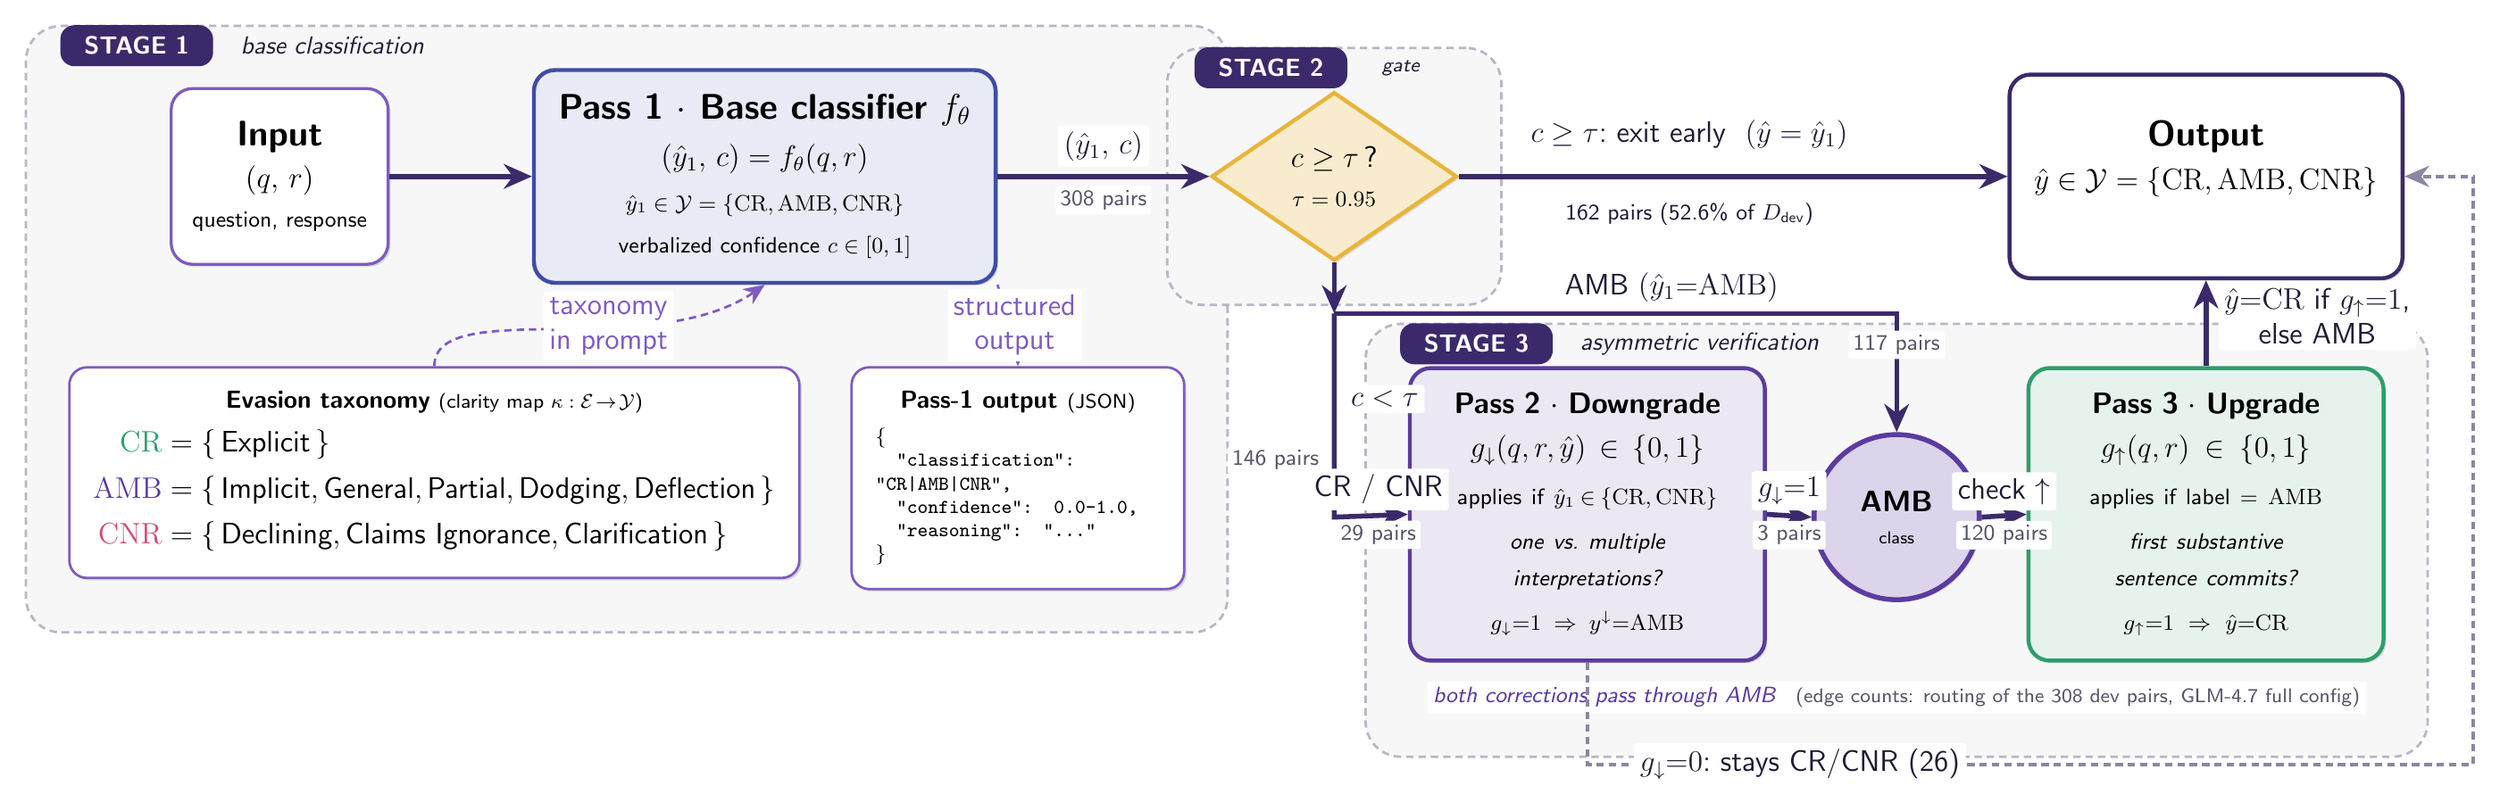
\begin{tikzpicture}[font=\large, every node/.style={font=\large}]

  % ---- figure-local styles (soft shadow; heavier weights; detail/hub/band/tab) ----
  \tikzset{
    softshadow/.style={drop shadow={shadow xshift=1pt, shadow yshift=-1pt, opacity=0.25}},
    io/.append style ={softshadow}, p1n/.append style={softshadow},
    % Pass 2 targets AMB: colour it with the AMB purple, not the CNR rose,
    % so box colours consistently encode the verifier's target class.
    p2n/.append style={softshadow, draw=purpleBrand, fill=ambColor!12},
    p3n/.append style={softshadow},
    % Output emits all three classes: neutral purple, not the CR green, so it
    % cannot be read as one unit with the green Pass-3 box directly below it.
    outn/.append style={softshadow, draw=purpleDeep, fill=white},
    io/.append style={fill=white},
    gate/.append style={softshadow},
    % no-op bypass reads as passive, not as an error path
    flf/.append style={draw=slateA},
    lbl/.append style={font=\large, inner sep=2.4pt, align=center},
    cnt/.style={font=\small, text=inkA!75, fill=white, inner sep=1.8pt,
                rounded corners=1pt, align=center},
    fl/.append style ={line width=2pt},
    flf/.append style={line width=1.6pt},
    detail/.style={rounded corners=2.5mm, draw=violetA, line width=1pt,
                   fill=white, align=center, inner sep=3.4mm, softshadow},
    hub/.style   ={circle, draw=purpleBrand, line width=2pt, fill=ambColor!22,
                   align=center, inner sep=0.4mm, softshadow},
    band/.style  ={rounded corners=5mm, draw=slateA!60, line width=1pt,
                   densely dashed, fill=slateA!7, inner sep=6mm},
    tab/.style   ={rounded corners=2mm, fill=purpleDeep, text=white,
                   font=\bfseries, inner xsep=3.4mm, inner ysep=1.7mm,
                   anchor=north west},
    sub/.style   ={anchor=west, font=\itshape, text=inkA},
    dfl/.style   ={-{Stealth[length=3mm,width=2.6mm]}, line width=1pt,
                   draw=violetA, densely dashed},
  }

  % =====================================================================
  %  MAIN SPINE  (happy path, common baseline y = 0):
  %  input -> classifier -> gate ......... output
  % =====================================================================
  \node[io,  minimum width=2.9cm, minimum height=2.5cm] (in) at (2.4,0)
        {{\ttl Input}\\[3pt]
         $(q,\,r)$\\[2pt]
         {\small question, response}};

  \node[p1n, minimum width=6.4cm, minimum height=2.9cm] (p1) at (9.3,0)
        {{\ttl Pass 1 $\cdot$ Base classifier $f_\theta$}\\[5pt]
         $(\hat y_1,\,c)=f_\theta(q,r)$\\[4pt]
         {\small $\hat y_1\in\mathcal Y=\{\mathrm{CR},\mathrm{AMB},\mathrm{CNR}\}$}\\[3pt]
         {\small verbalized confidence $c\in[0,1]$}};

  \node[gate, minimum width=3.4cm, minimum height=2.4cm] (gate) at (17.4,0)
        {$c \ge \tau\,$?\\[2pt]
         {\small $\tau=0.95$}};

  \node[outn, minimum width=5.2cm, minimum height=2.9cm] (out) at (29.8,0)
        {{\ttl Output}\\[4pt]
         $\hat y\in\mathcal Y=\{\mathrm{CR},\mathrm{AMB},\mathrm{CNR}\}$\\[3pt]
         {\Large\checkmark}};

  % =====================================================================
  %  STAGE 1 detail : evasion taxonomy as a clarity map + JSON cross-section
  %  (second-row grid; tops aligned at y = -2.7 via anchor=north)
  % =====================================================================
  % nine-subtype taxonomy as a formal, colour-coded map  kappa : E -> Y
  \node[detail, anchor=north] (tax) at (4.6,-2.7)
        {{\normalsize\bfseries Evasion taxonomy}\;%
           {\footnotesize(clarity map $\kappa:\mathcal E\!\to\!\mathcal Y$)}\\[5pt]
         $\begin{aligned}
            \textcolor{crColor}{\mathrm{CR}}   &= \{\,\text{Explicit}\,\}\\[1.5pt]
            \textcolor{ambColor}{\mathrm{AMB}} &= \{\,\text{Implicit},\text{General},
                     \text{Partial},\text{Dodging},\text{Deflection}\,\}\\[1.5pt]
            \textcolor{cnrColor}{\mathrm{CNR}} &= \{\,\text{Declining},
                     \text{Claims Ignorance},\text{Clarification}\,\}
          \end{aligned}$};

  % JSON "cross-section" of the Pass-1 output (monospace)
  \node[detail, anchor=north] (json) at (12.9,-2.7)
        {{\normalsize\bfseries Pass-1 output}\ {\footnotesize(JSON)}\\[5pt]
         \begin{minipage}{4.05cm}\ttfamily\footnotesize\raggedright
           \{\\
           \ \ "classification": "CR|AMB|CNR",\\
           \ \ "confidence": 0.0-1.0,\\
           \ \ "reasoning": "\ldots"\\
           \}
         \end{minipage}};

  \draw[dfl] (tax.north) .. controls +(0,1.0) and +(-1.6,-1.1) .. (p1.south)
        node[lbl, pos=0.62, text=violetA] {taxonomy\\ in prompt};
  \draw[dfl] (p1.south east) .. controls +(0.3,-1.1) and +(0,1.1) .. (json.north)
        node[lbl, pos=0.44, text=violetA] {structured\\ output};

  % =====================================================================
  %  STAGE 3 spine  (asymmetric verification, centres at y = -4.5):
  %  downgrade  ->  AMB hub  ->  upgrade
  % =====================================================================
  \node[p2n, anchor=north, text width=4.35cm, minimum height=3.6cm] (pd) at (21.0,-2.7)
        {{\vtl Pass 2 $\cdot$ Downgrade}\\[4pt]
         $g_\downarrow(q,r,\hat y)\in\{0,1\}$\\[5pt]
         {\small applies if $\hat y_1\!\in\!\{\mathrm{CR},\mathrm{CNR}\}$}\\[4pt]
         {\small\itshape one vs.\ multiple}\\[1pt]
         {\small\itshape interpretations?}\\[4pt]
         {\small $g_\downarrow{=}1\Rightarrow y^{\downarrow}{=}\mathrm{AMB}$}};

  \node[hub, minimum size=2.35cm] (amb) at (25.4,-4.85)
        {\textbf{AMB}\\[-1pt]{\scriptsize class}};

  \node[p3n, anchor=north, text width=4.35cm, minimum height=3.6cm] (pu) at (29.8,-2.7)
        {{\vtl Pass 3 $\cdot$ Upgrade}\\[4pt]
         $g_\uparrow(q,r)\in\{0,1\}$\\[5pt]
         {\small applies if label $=\mathrm{AMB}$}\\[4pt]
         {\small\itshape first substantive}\\[1pt]
         {\small\itshape sentence commits?}\\[4pt]
         {\small $g_\uparrow{=}1\Rightarrow \hat y{=}\mathrm{CR}$}};

  \node[font=\small\itshape, text=purpleBrand, align=center,
        fill=white, inner sep=2.5pt, rounded corners=1pt] (cap)
        at ($(pd.south)!0.5!(pu.south)+(0,-0.5)$)
        {both corrections pass through AMB\;\;
         {\footnotesize\upshape\color{inkA!75}(edge counts: routing of the 308 dev pairs, GLM-4.7 full config)}};

  % =====================================================================
  %  EDGES
  % =====================================================================
  % ---- spine 1->2 ----
  \draw[fl] (in) -- (p1);
  \draw[fl] (p1) -- (gate) node[lbl, midway, above=1mm] {$(\hat y_1,\,c)$}
        node[cnt, midway, below=1mm] {308 pairs};

  % ---- gate: early exit straight across the top baseline ----
  \draw[fl] (gate.east) -- (out.west)
        node[lbl, pos=0.42, above=2.6mm] {$c\ge\tau$:\ exit early\ \ $(\hat y=\hat y_1)$}
        node[lbl, pos=0.42, below=2.6mm] {\small 162 pairs (52.6\% of $D_{\text{dev}}$)};

  % ---- gate: low-confidence drop, then split by predicted class ----
  \coordinate (J)   at (17.4,-1.95);        % branch point below the gate
  \draw[fl] (gate.south) -- (J);

  % CR/CNR : straight down to the stage-3 baseline, into the downgrade verifier
  % (routing counts let the flow reconcile: 146 = 29 + 117; 120 = 117 + 3)
  \draw[fl] (J) -- (17.4,-4.85) node[lbl, pos=0.42, right=1.2mm] {$c<\tau$}
                                node[cnt, pos=0.72, left=1.2mm] {146 pairs}
                -- (pd.west)    node[lbl, pos=0.60, above=0.4mm] {CR / CNR}
                                node[cnt, pos=0.60, below=0.4mm] {29 pairs};

  % AMB (from Pass 1) : bus above the downgrade box, straight into the AMB hub
  \draw[fl] (J) -| (amb.north)
        node[lbl, pos=0.30, above=0.4mm] {AMB $(\hat y_1{=}\mathrm{AMB})$}
        node[cnt, pos=0.55, below=0.4mm] {117 pairs};

  % ---- downgrade outcome: g=1 routes into the AMB hub ----
  \draw[fl] (pd.east) -- (amb.west)
        node[lbl, midway, above=0.4mm] {$g_\downarrow{=}1$}
        node[cnt, midway, below=0.4mm] {3 pairs};

  % ---- AMB hub feeds the upgrade verifier ----
  \draw[fl] (amb.east) -- (pu.west)
        node[lbl, midway, above=0.4mm] {check $\uparrow$}
        node[cnt, midway, below=0.4mm] {120 pairs};

  % ---- upgrade result -> output (straight up the shared column) ----
  \draw[fl] (pu.north) -- (out.south)
        node[lbl, pos=0.58, right=1.4mm] {$\hat y{=}\mathrm{CR}$ if $g_\uparrow{=}1$,\\ else AMB};

  % ---- pass-2 "stays" : dashed bypass under stage 3, up the far right, into
  %      output.east (keeps the arrowhead clear of the pu.north -> out.south edge) ----
  \draw[flf] (pd.south) -- ++(0,-1.45)
        -| (33.6,0) node[lbl, pos=0.12] {$g_\downarrow{=}0$:\ stays CR/CNR (26)}
        -- (out.east);

  % =====================================================================
  %  STAGE BANDS  (drawn behind everything) + labelled tabs
  % =====================================================================
  \begin{scope}[on background layer]
    \node[band, fit=(in)(p1)(tax)(json)]     (b1) {};
    \node[band, fit=(gate)]                  (b2) {};
    \node[band, fit=(pd)(amb)(pu)(cap)]      (b3) {};
  \end{scope}

  \node[tab] at ($(b1.north west)+(0.5,0.0)$) {STAGE 1};
  \node[sub] at ($(b1.north west)+(2.95,-0.30)$) {base classification};
  \node[tab] at ($(b2.north west)+(0.4,0.0)$) {STAGE 2};
  \node[sub, font=\itshape\footnotesize] at ($(b2.north west)+(2.95,-0.30)$) {gate};
  \node[tab] at ($(b3.north west)+(0.5,0.0)$) {STAGE 3};
  \node[sub] at ($(b3.north west)+(2.95,-0.30)$) {asymmetric verification};

\end{tikzpicture}
\end{document}
